
%-----------------------------------------------------------------------------
\chapter{Epistatic GWAS analysis\label{ch:gwas}}
%-----------------------------------------------------------------------------

%---
\section{Preface}
%---

In recent years over 80 genetic loci related to type II diabetes (T2D) have been identified \cite{morris2012large, consortium2014genome}.
However the combined effect sizes of all these loci account for less than 10\% of the overall disease predisposition \cite{manolio2009finding}. 
This poses the question of why, given that so much efforts has been directed at finding the genetic components of this disease, the loci found so far have such modest effects. 
The lack of large genetic effects is known as the ``missing heritability" problem and does not only arise in T2D but also in almost all complex traits. 
Recent studies on the topic of missing heritability \cite{zuk2012mystery, zuk2014searching} suggest that genetic interactions (a.k.a. epistasis) might be at least partly responsible for this issue.

In this chapter, we propose a novel framework that takes into account putative epistatic interactions in the context of genome wide association studies (GWAS) to uncover potentially interacting variants that might affect disease risk. 
Although in the computational approaches we describe is applicable to any complex trait, in this chapter we apply it to diabetes GWAS data.
Type II diabetes (T2D) is a complex disease that was first described by the Egyptians in 1500 BCE. Later the Greeks in 230 BCE used the term ``diabetes" meaning ``pass through" (or ``siphon") denoting the constant thirst and frequent urination of the patients. In the 1700s the term ``mellitus" (from honey) was added to denote that the urine was sweet and would ``attracts ants".

Diabetes symptoms include frequent urination, thirst, and constant hunger, high blood sugar (hyperglycemia) and insulin resistance. 
Long term complication from T2D may include eyesight problems, heart disease, strokes and kidney failure. 
Type II diabetes is highly correlated with obesity and disease rate has increased dramatically during the last 50 years. 
According to the World Health Organisation the prevalence of diabetes is around 8\% to 9\% in adults and an estimated 1.5 millions deaths were caused by diabetes in 2012 \cite{guariguata2014global}, which is predicted to be the 7th leading cause of death by 2030. 
The costs associated to treating diabetes patients in the U.S. alone are estimated around \$245 billion dollars.

The rest of the chapter is from the following paper: \textbf{P. Cingolani}, R. Sladek, M. Blanchette, ``A co-evolutionary approach for detecting epistatic interactions in genome-wide association studies", to be submitted to PLOS Computational Biology.

%---
\section{Abstract}
%---

\paragraph{Motivation} Epistasis, broadly defined as genetic interactions, is one of the likely factors explaining variants identified to date by why genome-wide association studies (GWAS) account for a small portion of heritable risk for complex diseases. Due to their high complexity, reduced statistical power and sometimes prohibitive computational requirements, epistatic GWAS have rarely been performed. 

\paragraph{Methods} In this paper, we propose a novel methodology for identifying putative epistatic interactions by combining interspecies comparison and population level variation. 
Using crystal structures for individual proteins and for complexes as well as genome wide multiple species alignment, we create a co-evolutionary substitution model that allows the calculation of the posterior probability of physical interaction between residues. 
These probabilities are then used as the interaction priors for an epistatic GWAS analysis using a Bayesian framework. 

\paragraph{Results} Our algorithms can be applied to genome wide scale sequencing studies for tens of thousands of samples, that typically yield millions of variants. 
We applied our approach to a large type II diabetes (T2D) case-control cohort and inferred a number of putative interactions associated with increased risk of developing T2D. 

\paragraph{Availability} Our code is publicly available at \texttt{github.com/pcingola/Epistasis}

%---
\section{Introduction}
%---

Genetic studies aim to discover how a phenotype of interest, such as disease risk or height, is affected by in individual's genetic background. 
Genome wide association studies (GWAS) are powerful techniques aimed at finding statistical associations between a phenotype and genetic variants \cite{clarke2011basic}. 
Although several genetic variants related to different phenotypes have been found, variants discovered in GWAS so far can only explain a small part for the phenotypic heritability of complex traits. 
For instance, all genetic variants associated to height collectively account for few centimetres in the offspring's height \cite{wood2014defining}.
Similarly the known variants related to type 2 diabetes risk collectively explain only 5\% to 10\% of the overall variance in disease predisposition \cite{morris2012large, consortium2014genome}. 
This problem is known as ``missing heritability" \cite{manolio2009finding} and recent theories suggest that genetic interactions (epistasis) might play an important role in it \cite{zuk2012mystery, zuk2014searching}.

The foundations for epistasis \cite{gao2010classification} have been proposed almost a hundred years ago by Bateson (1909) and Fisher (1918). 
It was the latter who coined the term to denote a ``statistical deviation of multi-locus genotype values from an additive linear model for the value of a phenotype" \cite{gao2010classification}. 
There is evidence of such interactions being involved in complex diseases. For instance an interaction between BACE1 and APOE4 having a significant association with Alzheimer's disease has consistently been replicated in different studies \cite{combarros2009epistasis}. 
Many types of situations can lead to epistatic interactions, perhaps the most common involves pairs of variants that encode amino acids whose physical interactions is required for their respective proteins to function in a pathway.

One of the main problems in finding association between interactions and disease is that out of the whole set of molecular interactions (the interactome) only a small part of it has been characterized \cite{venkatesan2009empirical}. 
Interacting proteins can be identified experimentally through several types of approaches (yeast two hybrid, protein fragment complementation assay, glutathione-s-transferase, affinity purification coupled to mass spectrometry, tandem affinity purification, etc. \cite{shoemaker2007deciphering}) and large databases of protein-protein interactions are now available for human \cite{stark2006biogrid, shoemaker2007deciphering}. 
In almost all cases, these methods identify the presence of an interaction between proteins but do not discern the exact residues mediating such interactions. Furthermore, it is estimated that up to 80\% of the human protein-protein interactions remains unknown \cite{venkatesan2009empirical}.

These issues can be partially addressed using computational predictions of either pairs of interacting proteins or interacting residues \cite{shoemaker2007decipheringP2}. 
A type of approaches that has been gaining popularity recently is one that makes use of the plethora of genomic sequences available for species other than human in order to discover evolutionary evidence of selective pressure on pairs of residues to identify interacting sites and interfaces \cite{marks2012protein}. 
Interacting residues and their neighbours may then be subject to compensating epistasis, where a mutation at a residue in one protein may be compensated by another mutation at a residue in the second protein \cite{pazos1997correlated}.
This is a phenomenon generically known as co-evolution. 
For example assuming that evolutionary pressure acts on both interaction sites simultaneously, co-occurring compensatory mutations can become fixed in the population with higher probability than non-compensatory ones. 
In light of this hypothesis, one can use statistical methods to analyse multiple sequence alignments of proteins from different organisms to find co-evolving sites. 
This types of approaches has been used to identify co-evolving sites both within a protein (e.g. N-terminal and C-terminal domains in PKG protein \cite{goh2000co}, GroES-L chaperoning system \cite{ruiz2013coevolution}, $\alpha$ and $\beta$ haemoglobin subunits \cite{pazos1997correlated}), and between interacting proteins (e.g. G-protein coupled receptors and protein ligands \cite{goh2000co}).

Many methods exist to find putative interaction loci, both within and across proteins, based on evolutionary evidence (see \cite{de2013emerging} for a review). 
The earliest methods for inferring co-evolution used either correlation or mutual information between two loci \cite{marks2012protein} in a multiple sequence alignment. 
However, these methods are known to have systematic biases due to the fact that they ignore phylogenetic relationships \cite{de2013emerging} or sequence heterogeneity problems \cite{weigt2009identification}. 
More sophisticated methods, such as DCA \cite{morcos2011direct}, PSICOV \cite{jones2012psicov} or mdMI \cite{clark2014multidimensional} try to overcome these biases by using global statistical models, however they are not suitable for GWAS-scale analysis for two main reasons. 
First, they require multiple alignments of a very large number of sequences (ranging from $400$ to $25L$, where $L$ is the length of the protein \cite{clark2014multidimensional}), and such depth remains only available for a small number of proteins. 
Second, they are computationally demanding (e.g. running for minutes or even days for each interacting pair of proteins being considered), making them unsuitable for analyses involving millions of variants spanning over thousands of proteins. 
Furthermore, a recent study shows that overall agreement between methods is not high (65\% or less) and predictive power is quite low (only 6\% of the ``top scoring pairs" are real interactions) \cite{clark2014multidimensional}.

Considering epistatic interactions in GWAS is challenging for several reasons: 
i) interaction models are by definition non-linear \cite{gao2010classification}; 
ii) analysing all order $N$ variant combinations requires great computational power and efficient algorithms or might just be infeasible because the number tests grows exponentially with $N$ \cite{phillips2008epistasis}; 
iii) multiple hypothesis testing correction can render association tests underpowered for all but very large cohorts \cite{gao2010classification, phillips2008epistasis}; and 
iv) there is no consensus of what genetic interaction means, which is reflected in the difficulty to find a unified model \cite{phillips2008epistasis,mani2008defining}. 
For all these reasons and due to the lack of sequencing cohorts large enough to detect these interactions, the application of epistatic models to sequencing studies has not been widespread. 
Furthermore, the required sample sizes to detect epistatic interactions depend on phenotypic effect size and variants' allele frequencies with some estimates assuming on the order of 10,000 to 500,000 cases \cite{jostins2013using} to be required. 
Such cohorts are now becoming feasible due to improvements and cost reductions in sequencing technology.

Approaches for epistatic GWAS do exist and they are based on a wide array of methodologies. 
In Zhao et alii \cite{zhao2006test}, the authors infer epistatic interaction probabilities by noting that interactions create linkage disequilibrium patterns in the disease population. 
A Bayesian framework in \cite{zhang2007bayesian} takes into account several risk models and uses Dirichlet priors to solve each model analytically, then they combine them in the full model posterior distribution calculated using an MCMC sampling technique. 
In Ackermann et alii \cite{ackermann2012systematic}, the authors look for over / under-represented allele pairs in a given population by performing an analysis of imbalanced allele pair frequencies. 
Finally, finding interacting variants can be viewed as an attribute selection problem, thus many machine learning methodologies have been proposed \cite{mckinney2006machine}. 
While all algorithms have relative advantages, there is no standard in epistatic GWAS analysis and we believe that better methods can be created by combining other sources of biological information, such as evolutionary evidence.

In this work we propose an approach to prioritize pairs of variants identified in case/control cohorts by combining genome wide association with epistatic interaction models. 
In a nutshell, our method uses recently computed 100-way vertebrate genome alignments \cite{blanchette2004aligning} to calculate interaction posterior probabilities for any given pair of residues in human proteins. 
This is achieved by contrasting the likelihood of the observed pair of alignment columns under a joint substitution model that factors in dependencies between interacting sites, and a null model of independent evolution. 
The posterior probabilities can then used as priors to modulate the evidence of epistatic interaction derived from GWAS data. 
Our implementation is efficient enough to be applied to GWAS-scale datasets of tens of thousands of samples. 
Finally we showcase this method using a cohort of $\sim 13,000$ individuals in a case-control study of type II diabetes (for study details, see \cite{mccarthy2015T2D}) and identify suggestive associations of putatively epistatic interactions.

%---
\section{Methods \label{sec:gwasMeth}}
%---

Our epistatic GWAS analysis pipeline involves three key steps, as shown in Figure \ref{fig:gwaspipeline}. 
First, we learn a co-evolutionary substitution rate matrix from pairs of amino acids that are known to be in contact within proteins. 
Second, we analyse a GWAS data set to identify pairs of non-synonymous variants that show (possibly weak) evidence of epistasis. 
Third, for each pair of variants identified in step 2, we measure the evidence of co-evolution of the pair of encoded amino acids, and combine it with the GWAS evidence by calculating a joint Bayes factor.

\fig{gwas_epistasis_pipeline}{gwaspipeline}{16cm}{Complete pipeline example}{Complete pipeline example}

\subsection{Substitution model for pairs of interacting amino acids \label{sec:gwasQ2}}

In this section, we describe how we estimate two substitution rate matrices:
i) the first is the usual $20 \times 20$ substitution rate matrix $Q$ describing the evolution of individual amino acids;
ii) the second, $Q_2$, is a $400 \times 400$ substitution rate matrix for pairs of interacting residues. 

We use the 100-way vertebrate multiple sequence alignment and accompanying phylogenetic tree $T$ available from the UCSC Genome Browser \cite{karolchik2014ucsc}. 
This alignment includes the DNA sequences of 100 species whose genome is completely or nearly completely sequenced, with 12 primates, 44 non-primates eutherians, 5 marsupials, 14 birds, 6 reptiles, 16 ray-finned fish and 8 lobe-fined fish.
The multiple alignment is performed using the multiz algorithm \cite{blanchette2004aligning,kielbasa2011adaptive}.

From the $\sim21,000$ human protein structures (resolution less than $3$ \r{A}) available in Protein Data Bank, we extracted a set of $\sim770,000$ pairs of ``within protein interactions" residues, defined as pairs of residues from the same protein where at least one pair of atoms is within $3$ \r{A}. 
Similarly, from the set of $\sim5,700$ models of co-crystallized complexes in PDB, we extracted a set of $\sim12,000$ pairs of ``protein-protein interacting" residues, defined as amino acids from different proteins that satisfy the same distance criterion.

To derive the rate matrix $Q$, we consider the complete set of $n \sim 22 \times 10^6$ protein coding sites present in the alignment, irrespective of the presence or absence of contacts. $Q$ is obtained following classical sequence evolution theory (\cite{yang2006computational, felsenstein2004inferring}). 
First, for each pair of species  $s_i$ and $s_j$, we obtain $c_i(a)$ defined as the count of amino acid $a$ in species $s_i$, and $c_{i,j}(a,b)$ defined as the number of sites that have had a transition from amino acid $a$ in $s_i$ to $b$ in $s_j$. 
Stationary probability of amino acid $a$ in genome $s_i$ is then defined as $\pi_i = c_i(a)/n$. 
Assuming a time reversible model, we get the frequency of change from $a$ to $b$: $f_{i,j}(a,b) = f_{j,i}(a,b) = (c_{i,j}(a,b) + c_{j,i}(a,b))/(2n)$. Let $P_{i,j}$ be the amino acid transition probability matrix from $s_i$ to $s_j$, i.e. $P_{i,j}(a,b)$ is the probability that species $s_j$ has amino acid $b$ given that species $s_i$ has amino acid $a$. 
Then $P_{i,j}$ is obtained through the relation $f_{i,j}(a,b) = \pi_i(a) \cdot P_{i,j}(a,b)$, or $P_{i,j}(a,b) =   f_{i,j}(a,b) /  \pi_i(a)$. 
Let $t_{i,j}$ be the total branch length between $s_i$ and $s_j$ (obtained from the phylogenetic tree). 
Assuming time reversibility, we have $P_{i,j} = e^{Q \cdot t_{i,j}}$, and thus $Q=log[ P_{i,j} / t_{i,j} ]$ \cite{yang2006computational}. 
Taking into account the estimation error, the equation becomes $\hat{Q}_{i,j} = log[ P_{i,j} / t_{i,j} ] + \epsilon_{i,j}$, where $\epsilon_{i,j}$ is an error matrix. Under the assumption that the mean error is zero, we can approximate the rate matrix by the calculating an average of all estimates:

\begin{eqnarray*}
	\hat{Q} & = & \frac{1}{N(N-1)/2} \sum_{i < j} \hat{Q}_{i,j} \\
	            & =  & \frac{2}{N(N-1)} \sum_{i<j} \frac{1}{t_{i,j}} log[ \hat{P}_{i,j} ]
\end{eqnarray*}

The much larger substitution matrix $Q_2$ describes the substitution rate from any pair of amino acids $(a,b)$ to any other pair $(c,d)$. 
It is derived similarly to $Q$, but considering only pairs of amino acids from the set of within protein interacting pairs of amino acids. 
We only take into account amino acids pairs within the same chain, that are separated by 20 amino acids or more. 

\subsection{Calculating likelihood of individual and pairs of alignment columns}

Given a substitution rate matrix $Q$, a multiple sequence alignment $MSA$, and a phylogenetic tree $T$ for the sequences in $MSA$, the likelihood of an alignment column $MSA(i)$ (i.e. $L_1[MSA(i)]$) can be calculated using Felsenstein's algorithm \cite{felsenstein2004inferring}, which has a time complexity of $O(N \cdot |\Sigma|^2)$, where $|\Sigma|=20$ is the alphabet size and $N$ is the number of sequences in the alignment. 
Given matrix $Q_2$, the same algorithm can be used to compute the likelihood $L_2[ MSA(i), MSA(j) ]$ of a pair of alignment columns $( MSA(i), MSA(j) )$, but now in time $O(N \cdot |\Sigma|^4)$. 

A test for co-evolution of two positions $i$, $j$ from the same or different proteins is obtained from the log-likelihood ratio of these two models: 
%\begin{eqnarray*}
%	L_C[MSA(i), MSA(j)] = \frac{L_2[ MSA(i), MSA(j) ]}{L_1[MSA(i)] \cdot L_1[MSA(j)]}
%\end{eqnarray*}
%
%Similarly, the log-likelihood is defined as
%
\begin{eqnarray}
    \ell_C[MSA(i), MSA(j)] = log \left[ \frac{L_2[ MSA(i), MSA(j) ]}{L_1[MSA(i)] \cdot L_1[MSA(j)]} \right]
\end{eqnarray}
\noindent where the denominator assumes that the amino acids $i$ and $j$ evolve independently. 

In a GWAS study these likelihood calculations need to be performed on a very large number of pairs of sites, thus optimizations are required to ensure manageable running time. 
First, pre-calculation of  matrix exponentials $P(t) = e^{Qt}$ can be performed for all values of $t$ corresponding to individual branch lengths in the phylogenetic tree $T$. 
Second, ``constant-tree caching" is used to cache likelihood values for sub-trees of the phylogenetic tree where all nodes have the same amino acid 
% values; obviously for this optimization to result in a meaningful speed-up the phylogenetic tree $T$ should remain constant throughout the genome, which is the case in our model.

\subsection{GWAS model}

Consider a GWAS with $N_S$  samples (individuals) and $N_V$ variants, we use the standard notation for phenotypes and code them as $d_s=1$ when individual $s$ is affected by disease (cases) and $d_s=0$ if the individual is ``healthy" (control). 
Let $\bar{d} = [d_1, ..., d_{N_s}]$ be a phenotype vector and $g_{s,i} \in \{0,1,2\}$ a genomic variant for sample $s$ at locus $i$. A logistic model of disease risk \cite{balding2006tutorial} is
\begin{eqnarray*}
    p_{s,i} & = & P( d_s=1 | g_{s,i}, \bar{\theta} ) \\
    & = & \phi( \theta_0 + \theta_1 g_{s,i} + \theta_2 c_{s,1} + \theta_4 c_{s,2} + ... ) \\
    & = & \frac{1}{1 + e^{-(\theta_0 + \theta_1 g_{s,i} + \theta_2 c_{s,1} + \theta_4 c_{s,2} + ...})} \\
    & = & \phi( \bar{\theta}^T \bar{g}_{s,i})
\end{eqnarray*}
\noindent where $\phi(\cdot)$ is the sigmoid function, $c_{s,1}, c_{s,2}, ... $ are covariates for each individual $s$ (these covariates usually include sex, age and eigenvalues from population structure analysis \cite{price2006principal}), $\bar{g}_{s,i} = [ 1, g_{s,i} , c_{s,1}, c_{s,2}, ... , c_{s,N_C} ]$, and $\bar{\theta} = [\theta_1, \theta_2, ..., \theta_m] $. 
The parameter estimates $\bar{\theta}$ are obtained by solving the maximum likelihood equation
\begin{eqnarray*}
    L( \bar{\theta} ) & = & \prod_{s=1}^{N_S}{ P( d_s | \bar{\theta}, g_{s,i} ) } \\
    & = & \prod_{s=1}^{N_S}{ p_{s,i}^{d_s} (1-p_{s,i})^{1-d_s} } \\
    & = & \prod_{s=1}^{N_S}{ \phi( \bar{\theta}^T \bar{g}_{s,i})^{d_s} (1-\phi( \bar{\theta}^T \bar{g}_{s,i}))^{1-d_s} }
\end{eqnarray*}
Using this model, we have two hypotheses: 
i) the null hypothesis, $H_0$, assumes that genotype does not influence disease probability (i.e. $\theta_1 = 0$); and
ii) the alternate hypothesis, $H_1$, assumes that the genotype does influence disease probability (i.e. $\theta_1 \neq 0$). 
We can compare these two hypotheses using a likelihood ratio test, so we define
\begin{eqnarray*} \label{eq:gwasLogLikLogReg}
	% L_G & = & \frac{L( \bar{\theta} | H_1 ) }{ L( \bar{\theta}' | H_0 ) }\\
	\ell_G & = & log \left[ \frac{L( \bar{\theta} | H_1 ) }{ L( \bar{\theta}' | H_0 ) } \right]
\end{eqnarray*}
\noindent where $\bar{\theta}'$ and $\bar{\theta}$ are the maximum likelihood estimates for null and alternate models respectively. 
According to Wilk's theorem \cite{wilks1938large}, the log likelihood ratio has a $\chi^2_1$ distribution under the null hypothesis, so we can easily calculate a p-value.

Next, we extend the logistic model to accommodate interacting loci. For an individual (sample $s$), we model interactions between two genetic loci $i$ and $j$, having genotypes $g_{s,i}$ and $g_{s,j}$, by extending the logistic model
\begin{eqnarray} \label{eq:gwasLogRegH1}
    P( d_s | g_{s,i},g_{s,j}, H_1) & = & \phi[ \theta_0 + \theta_1 g_{s,i} + \theta_2 g_{s,j} + \theta_3 (g_{s,i} g_{s,j}) \\
    & & ... + \theta_4 c_{s,1} + ... + \theta_m c_{s,N_{cov}} ] \\
    & = & \phi( \bar{\theta}^T \bar{g}_{s,i,j}) )
\end{eqnarray}
\noindent where $\bar{g}_{s,i,j} =  [1, g_{s,i}, g_{s,j}, ( g_{s,i} g_{s,j}), c_{s,1}, c_{s,2}, ..., c_{s,N_{cov}} ]^T$. 
An implicit assumption in this equation is that $g_{s,i}$ and $g_{s,j}$ are not correlated (e.g. they are not located in the same LD-Block). 
This can be enforced either by using haplotype structure information (e.g. from HapMap) or by limiting the application of the model to variants either in different chromosomes or sufficiently distant (say $> 1MB$), we use the latter.
The null hypothesis $H_0$ assumes that variants act independently
\begin{eqnarray} \label{eq:gwasLogRegH0}
    P( d_s | g_{s,i},g_{s,j}, H_0) & = & \phi[ \theta_0' + \theta_1' g_{s,i} + \theta_2' g_{s,j} + \theta_3' c_{s,1} + ... ] \\
   & = & \phi( \bar{\theta'}^T \bar{g}_{s,i,j}' )
\end{eqnarray}
\noindent where $\bar{g}_{s,i,j}' =  [1, g_{s,i}, g_{s,j}, c_{s,1} , c_{s,2}, ..., c_{s,N_{cov}} ]^T$.

Just as in the single loci, this requires fitting the logistic regression parameters, thus we investigated several algorithms for logistic regression parameter fitting. 
The fastest convergence is obtained using Iterative Reweighted Least Squares (IRWLS \cite{daubechies2010iteratively}) and Broyden-Fletcher-Goldfarb-Shanno algorithm (BFGS \cite{broyden1970convergence}) with some code optimizations. In most cases, IRWLS converges faster, so it was selected as the default implementation in our analysis.

Another way to compare the null hypothesis to the alternative hypothesis, is using a Bayesian formulation \cite{kass1995bayes, wakefield2009bayes}
\begin{eqnarray*}
	P(H_1 | \mathcal{D}) & = & \frac{ P( \mathcal{D} | H_1) P(H_1) }{ P(\mathcal{D}) } = \frac{ \int{ P(\mathcal{D} | \bar{\theta} , H_1) P( \bar{\theta} | H_1) P(H_1)  d\bar{\theta} } }{ P(\mathcal{D}) }  \\
	\Rightarrow  \frac{ P(H_1 | D)  }{ P(H_0 | D)  } & = & \frac{ \int{ P(\mathcal{D} | \bar{\theta} , H_1) P( \bar{\theta} | H_1)  d\bar{\theta} } }{\int{ P(\mathcal{D} | \bar{\theta'} , H_0 ) P( \bar{\theta'} | H_0)  d\bar{\theta'} } } \frac{ P(H_1) }{ P(H_0)  }  
	=  BF \frac{ P(H_1) }{ P(H_0)  }
\end{eqnarray*}
\noindent where $BF$, the ratio of the two integrals, is the Bayes factor. 
Using a Bayesian formulation has two main advantages: 
i) the hypothesis are automatically corrected for model complexity since Bayes factor asymptotically converges to Bayesian Information Criteria (BIC) \cite{kass1995bayes}, and 
ii) we can compare non-nested models. 
The Bayes factor for the epistatic model becomes:
\begin{eqnarray}\label{eq:bf2}
	BF_G = \frac
	{ \int{ \prod_{s=1}^{N_S}{ \phi( \bar{\theta}^T \bar{g}_{s,i,j})^{d_s} [ 1-\phi( \bar{\theta}^T \bar{g}_{s,i,j}) ]^{1-d_s} } P( \bar{\theta} | H_1)  d\bar{\theta} } }
	{ \int{ \prod_{s=1}^{N_S}{ 
	\phi( \bar{\theta'}^T \bar{g'}_{s,i,j} ) )^{d_s} 
	[ 1-\phi( \bar{\theta'}^T \bar{g'}_{s,i,j}) ]^{1-d_s} } 
	P( \bar{\theta'} | H_0)  
	d\bar{\theta'} } }
\end{eqnarray}
Calculating Bayes factors is challenging because most of the times there are no closed form equations and even if the integrals can be computed by means of numerical algorithms, it imposes a significant computational burden thus making it impractical for large datasets such as GWAS data.
We can approximate the integrals using Laplace's method  \cite{kass1995bayes}. If $g(x)$ has a maximum at $x_0$, it can be shown that
\begin{eqnarray*}
	\int{e^{-\lambda g(x)} h(x) dx} & \simeq & h(x_0) e^{\lambda g(x_0)} \sqrt{\frac{2 \pi}{\lambda g''(x_0)}} \\
\end{eqnarray*}
The multivariate case for $\bar{x} \in \Re^d$ is an analogous extension that uses a Hessian matrix instead of a second derivative of $g(\cdot)$
\begin{eqnarray}\label{eq:laplace}
	\int{e^{\lambda g(\bar{x})} h(\bar{x}) d\bar{x}} & \simeq & h(\bar{x}_0) e^{\lambda g(\bar{x}_0)} 
	\left( \frac{2 \pi}{\lambda} \right)^{d/2} \left[ \frac{\partial^2 g(\bar{x}) }{\partial \bar{x} \partial \bar{x}^T} \right] ^{-1/2}
\end{eqnarray}
Using equation \ref{eq:laplace} we can try to approximate the improper integrals in equation \ref{eq:bf2} by the transformation $L(\bar{\theta}) = e^{\ell(\bar{\theta})}$, where $\ell(\cdot)$ is the log-likelihood of the data, so we can use Laplace approximation by applying Eq.\ref{eq:laplace} at the point of the maximum likelihood.
In order to do so, we need to calculate the Hessian matrix in Eq.\ref{eq:laplace}.
Fortunately in logistic models 
%a few simplifications can be made by considering that $L(\bar{\theta}) = \prod_{s=1}^{N_S}{ \phi( \bar{\theta}^T \bar{g}_s)^{d_s} [ 1-\phi( \bar{\theta}^T \bar{g}_s) ]^{1-d_i} }$, so 
, it can be shown that for genotype terms
\begin{eqnarray*}
	\frac{ \partial^2 \ell(\bar{\theta}) }{ \partial\theta_i \partial\theta_j } 
	= \sum_s{ g_{s,i} g_{s,j} p_s (1-p_s) } 
\end{eqnarray*}
\noindent Using analogous derivation for the covariates, we can find an analytic form of the Hessian, which completes the Laplace approximation formula.

Calculating Bayes factors involves using prior parameter distributions. 
In order to estimate these distributions, we run the logistic regression fitting analysis and plot the parameter distributions for different levels of significance. 
As expected most parameters have uni-modal distribution, except for $\theta_3$, which has a multi-modal distribution. 
For all parameters, except $\theta_3$, we use a normal distribution centred at the mean and variance set to one ($\sigma=1)$ even though most times the variance is much smaller. 
This is done to avoid penalizing outliers too heavily and to have smooth derivatives near the maximum likelihood estimates. 
For $\theta_3$, which has a multi-modal distribution, we fit a mixture model parameters using an EM algorithm to fit a Gaussian bimodal.

\paragraph{Computational and statistical issues} 
The computational burden for the detection of pairs of interacting genetic loci affecting disease risk is significantly larger than in a standard (single variant) GWAS study. 
A priori all pairs of variants should be analysed, thus significantly increasing the number of statistical tests. 
This also reduces the statistical power since the required p-value significance level would be orders of magnitude smaller. 
A na{\"i}ve approach would estimate that if a typical genetic sequencing study has $10^6$ variants, a GWAS on epistatic variants would square that number of statistical tests, thus p-values required for significance would be in the order of $0.05 / (10^6)^2 = 5 \cdot 10^{-14}$. 

Fortunately these numbers can be reduced significantly. 
First, in this study, we only concentrate on non-synonymous coding variants. 
Second, as required by our co-evolutionary model, only variants overlapping a multiple sequence alignment are taken into account (when several multiple sequence alignments overlapped a region, the alignment with the longest number of proteins was selected).
Third, if two variants $g_i$ and $g_j$ are such that the interaction term $(g_{s,i} g_{s,j})$ is zero in all samples, which usually happens for pairs of rare variants, then $BF_G = 1$. 
Fourth, if the variants and the epistatic term $[g_{s,i}, g_{s,j}, g_{s,i} g_{s,j}]$ are linearly dependent, the logistic regression equations are undetermined, so we skip such variant pairs. 
Fifth, if one of the variants has high allele frequency with respect to the other, all non-zero epistatic terms may lie in the same positions as non-zero genotypes from the low frequency variant, causing logistic regression estimates to artificially inflate the coefficients of the low frequency variant and the epistatic term thus creating an artificially high association (low p-value). 
So we filter out these variant pairs as well. 
Finally, we filter out all variants having Hardy-Weinberg p-value of less than $10^{-6}$, since these variants also artificially inflate the logistic regression coefficients.  
Once the results are obtained, we can focus on pure epistatic interactions (i.e. interactions with no marginal contribution from each independent loci) by further filtering results and keeping variant pairs whose alternative logistic model (see equation \ref{eq:gwasLogRegH1}) has small absolute values for $\theta_1$ and $\theta_2$ while having large absolute values for $\theta_3$, specifically we keep results if $|\theta_3| > K ( |\theta_1| + |\theta_2| )$ (based on empirical data, we set $K=3$). 

\subsection{Putting it all together}

In summary, we first calculate the transitions matrices for the Markov models ($Q$ and $Q_2$) based on observations from protein structures (PDB) and multiple sequence alignments (UCSC's 100-way). 
We analyse variants from genome sequencing data first by filtering only for non-synonymous variants, then analysing all possible pairs of variants and filtering out those that are unsuitable for further analysis.
% (e.g. in linear dependence, deviation from Hardy-Weinberg equilibrium having p-value less than $10^{-6}$, etc.). 
From the pairs of variants that pass filtering, we fit two logistic regression models (null and alternative hypothesis), then calculate a p-value using the log-likelihood ratio, and keeping pairs of variants having p-values below a predefined threshold ($10^{-6}$). 
These pairs of variants are then analysed under our co-evolutionary model, we find the corresponding columns in the multiple sequence alignment and calculate the likelihoods for the null and alternative models by means of Felsenstein's algorithm (using matrices $Q$ and $Q_2$ in respectively). 
Finally, likelihoods from co-evolutionary and logistic regression models are used to calculate the total Bayes Factor ($BF_T$) by means of Laplace's approximation:
%, we extract the co-evolutionary likelihoods from the integrals by assuming independence from genotypes and noting that the probabilities do not depend on $\theta$:
\begin{eqnarray*}\label{eq:bftot}
	BF_T & = & \frac
	{ \int{ \prod_{s=1}^{N_S}{ \phi( \bar{\theta}^T \bar{g}_{s,i,j})^{d_s} [ 1-\phi( \bar{\theta}^T \bar{g}_{s,i,j}) ]^{1-d_s} } P( \bar{\theta} | H_1)  d\bar{\theta} } }
	{ \int{ \prod_{s=1}^{N_S}{ 
	\phi( \bar{\theta'}^T \bar{g'}_{s,i,j} ) )^{d_s} 
	[ 1-\phi( \bar{\theta'}^T \bar{g'}_{s,i,j}) ]^{1-d_s} } 
	P( \bar{\theta'} | H_0)  
	d\bar{\theta'} } } \\
	& & \cdot \frac{L_2[ MSA(i), MSA(j) ]}{L_1[MSA(i)] \cdot L_1[MSA(j)]} \\
	BF_T & = & BF_G \cdot L_C
\end{eqnarray*}

%---
\section{Results}
%---

Our approach, which is summarized in Figure \ref{fig:gwaspipeline}, involves three main components. 
First we estimate evolutionary substitution rates for individual amino acids in a protein as well as for pairs of amino acids (either from the same protein or not) that are physically interacting.
Given a set of multiple protein sequence alignment these evolutionary models can be used as a statistical test for co-evolution between any two amino acids without using structural information. 
Second, a statistical test for epistasis is developed to identify pairs of non-synonymous variants that show (often weak) evidence of interaction in the way they associate to a given trait. 
Finally, evidence from the co-evolution model and the epistatic GWAS model are combined in a Bayesian framework.
 
\subsection{Co-evolutionary substitution models}

The approach described in Methods was used to obtain substitution rate matrices $Q$ for individual amino acids and $Q_2$ for pairs of physically interacting residues within the same protein. 
Unsurprisingly, $Q$ (or more precisely a transition matrix $P(t)$ obtained from $Q$) is very similar to well known transitions matrices such as PAM \cite{dayhoff1978model} (Supplementary Figure \ref{fig:gwas_Qhat_vs_PAM1}).

The structure of $Q_2$, which describes substitution rates between one pair of interacting amino acids to another, is richer (Supplementary Figure \ref{fig:gwas_Q2}). 
Of particular interest are pairs of amino acids having high ratio $R(ab,cd) = Q_2 (ab, cd) / ( Q(a,c) \cdot Q(b,d) )$ which is an indicative of co-evolution.
For example the highest ratio is found in amino acid pair transition \texttt{V.I -> W.W} (i.e. amino acid \texttt{V} mutated to \texttt{W} in one of the sequences, and amino acid \texttt{I} changed to \texttt{W} in the other). 
In fact all top 10 ratios are transitions to \texttt{W.W} amino acid pairs.
This makes sense considering that:
i) individual amino acid substitution rates to tryptophan are generally very low, but that 
ii) tryptophan pairs are well known $\beta$-hairpin stabilizers and are considered as a paradigm for designing stable $\beta$-hairpins \cite{santiveri2010tryptophan}.

Another type of pair transitions with large $R(ab,cd)$ ratio is the double transitions to a pair of phenylalanine amino acids from a pair of hydrophobic amino acids (Lysine, Asparagine, Glutamine, Arginine, Aspartic acid and Glutamic acid). 
Phenylalanine-Phenylalanine interaction pairs are assumed to conform $\pi-\pi$ interactions which are predicted and experimentally observed to be energetically favourable \cite{hunter1991pi}.

\subsection{Co-evolutionary model validation}

We first assessed the ability of our co-evolutionary model to detect interacting sites located within the same protein by computing the likelihood ratio of candidate pairs of sites under a co-evolutionary model ($Q_2$) versus under independence ($Q$). 
Although such pairs of sites are unlikely to exhibit evidence of epistasis in GWAS studies (due to linkage), accurate prediction of interacting sites in a given protein are useful for many other purposes, such as protein structure prediction and prediction of the impact of individual mutations.  
Figure \ref{fig:gwas_figure_2} shows that interacting sites tend to have higher likelihood ratio scores than non-interacting ones (Mann-Whitney p-value $< 2.2 \times 10^{-16}$). 
Although the likelihood ratio score by itself cannot perfectly discriminate between the two classes, only 25.9\% of non-interacting pairs have a likelihood ratio above the median likelihood ratio of interacting pairs. 

\fig{gwas_figure_2}{gwas_figure_2}{12cm}{Histogram of log-likelihood values of pairs of amino acids in contact (red) and not in contact (blue) for amino acids within the protein (PDB). Log-odds of contacting vs non-contacting pairs (black) and smoothed log-odds (dotted grey).}{Histogram of log-likelihood values of pairs of amino acids in contact vs not in contact (within protein).}

To confirm that a co-evolutionary model estimated on pairs of interacting sites from the same protein is useful at predicting pairs of interacting sites between proteins, we repeated the same type of analysis on $\sim3,000$ pairs of interacting ($< 3$ \r{A}) and $\sim3,000$ pairs of non-interacting ($>30$ \r{A}) residues from distinct proteins, obtained from co-crystal structures in PDB (see Methods). 
As seen on Figure \ref{fig:gwas_figure_3}, the two classes of sites have substantially different likelihood ratio distributions (Mann-Whitney one sided test: $p-value < 2.2 \times 10^{-16}$), although slightly less so than for sites from the same protein. Only 29\% of non-interacting sites have a likelihood ratio larger than the median for interacting sites. 
These empirical distributions allow us to approximate of the log odds of the ``interacting" vs ``non-interacting" amino acids distributions as
\begin{eqnarray*}
%O_{dds}(x) & = & \frac{P[ L_2(MSA(i), MSA(j)) \ge x ]}{P[ L_1(MSA(i) \times L_1(MSA(j) \ge x]} \\
\ell_{odds}(x) & = & log\left[ \frac{P[ L_2(MSA(i), MSA(j)) \ge x ]}{P[ L_1(MSA(i) \times L_1(MSA(j) \ge x]} \right] \\
    & \simeq &e^{\alpha x}- \beta \\
\end{eqnarray*}
\noindent where $\alpha = 0.195$ and $\beta = 1.018$ (in order to avoid biases, the log odds value is capped to $4.0$).

\fig{gwas_figure_3}{gwas_figure_3}{12cm}{
Histogram of log-likelihood values of pairs of amino acids in contact (red) and not in contact (blue) for amino acids in different proteins (co-crystallized entries from PDB). 
Log-odds of contacting vs non-contacting pairs (black) and smoothed log-odds (dotted grey)}{Histogram of log-likelihood values of pairs of amino acids in contact vs not in contact (co-crystallized proteins)}

Figure \ref{fig:gwas_jmol} shows the example of a predicted contact $\ell_C = 7.7$ between \textit{Senp1} and \textit{Sumo1} proteins detected by our method. The co-crystallized structure from PDB highlights the interacting amino acids (less than $3$ \r{A} apart) and the corresponding multiple alignment columns.

Although our approach aims at identifying contacting residues from different proteins, it can also be used to predict the presence or absence of interactions between proteins as a whole. 
We extracted from BioGrid \cite{stark2006biogrid} a set of $\sim3,000$ pairs of human proteins with evidence of interaction, and further required that both proteins belong to the same pathway (MsigDb, C2 groups \cite{subramanian2005gene}), and their corresponding genes are expressed in the same tissue (GTex \cite{lonsdale2013genotype}, expression of 1 FPKM or more, tissues $\in$ \{skeletal muscle, adipose tissue, pancreatic Islets\}). We randomly selected as ``non-interacting" pairs the same number of pairs amongst those that do not fulfil any of the three conditions.

\begin{figure}[p]
%\centering
\begin{subfigure}[t]{0.7\textwidth}
  \centering
  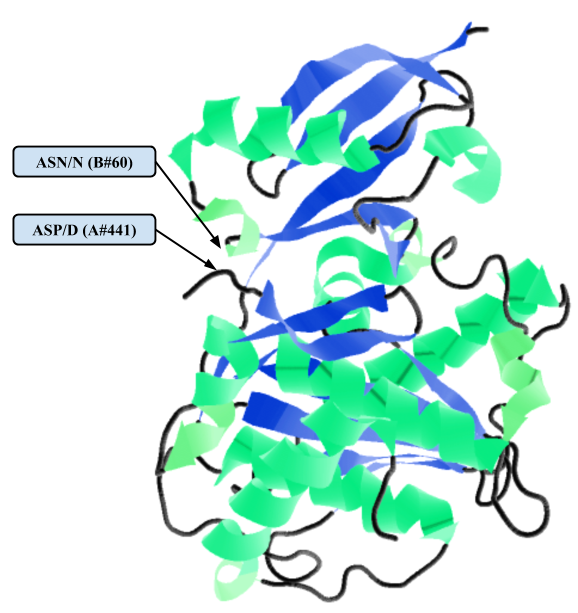
\includegraphics[height=10cm]{figs/gwas_figure_4_jmol.png}
  \label{fig:sub1}
\end{subfigure}
\begin{subfigure}[t]{.2\textwidth}
  \centering
  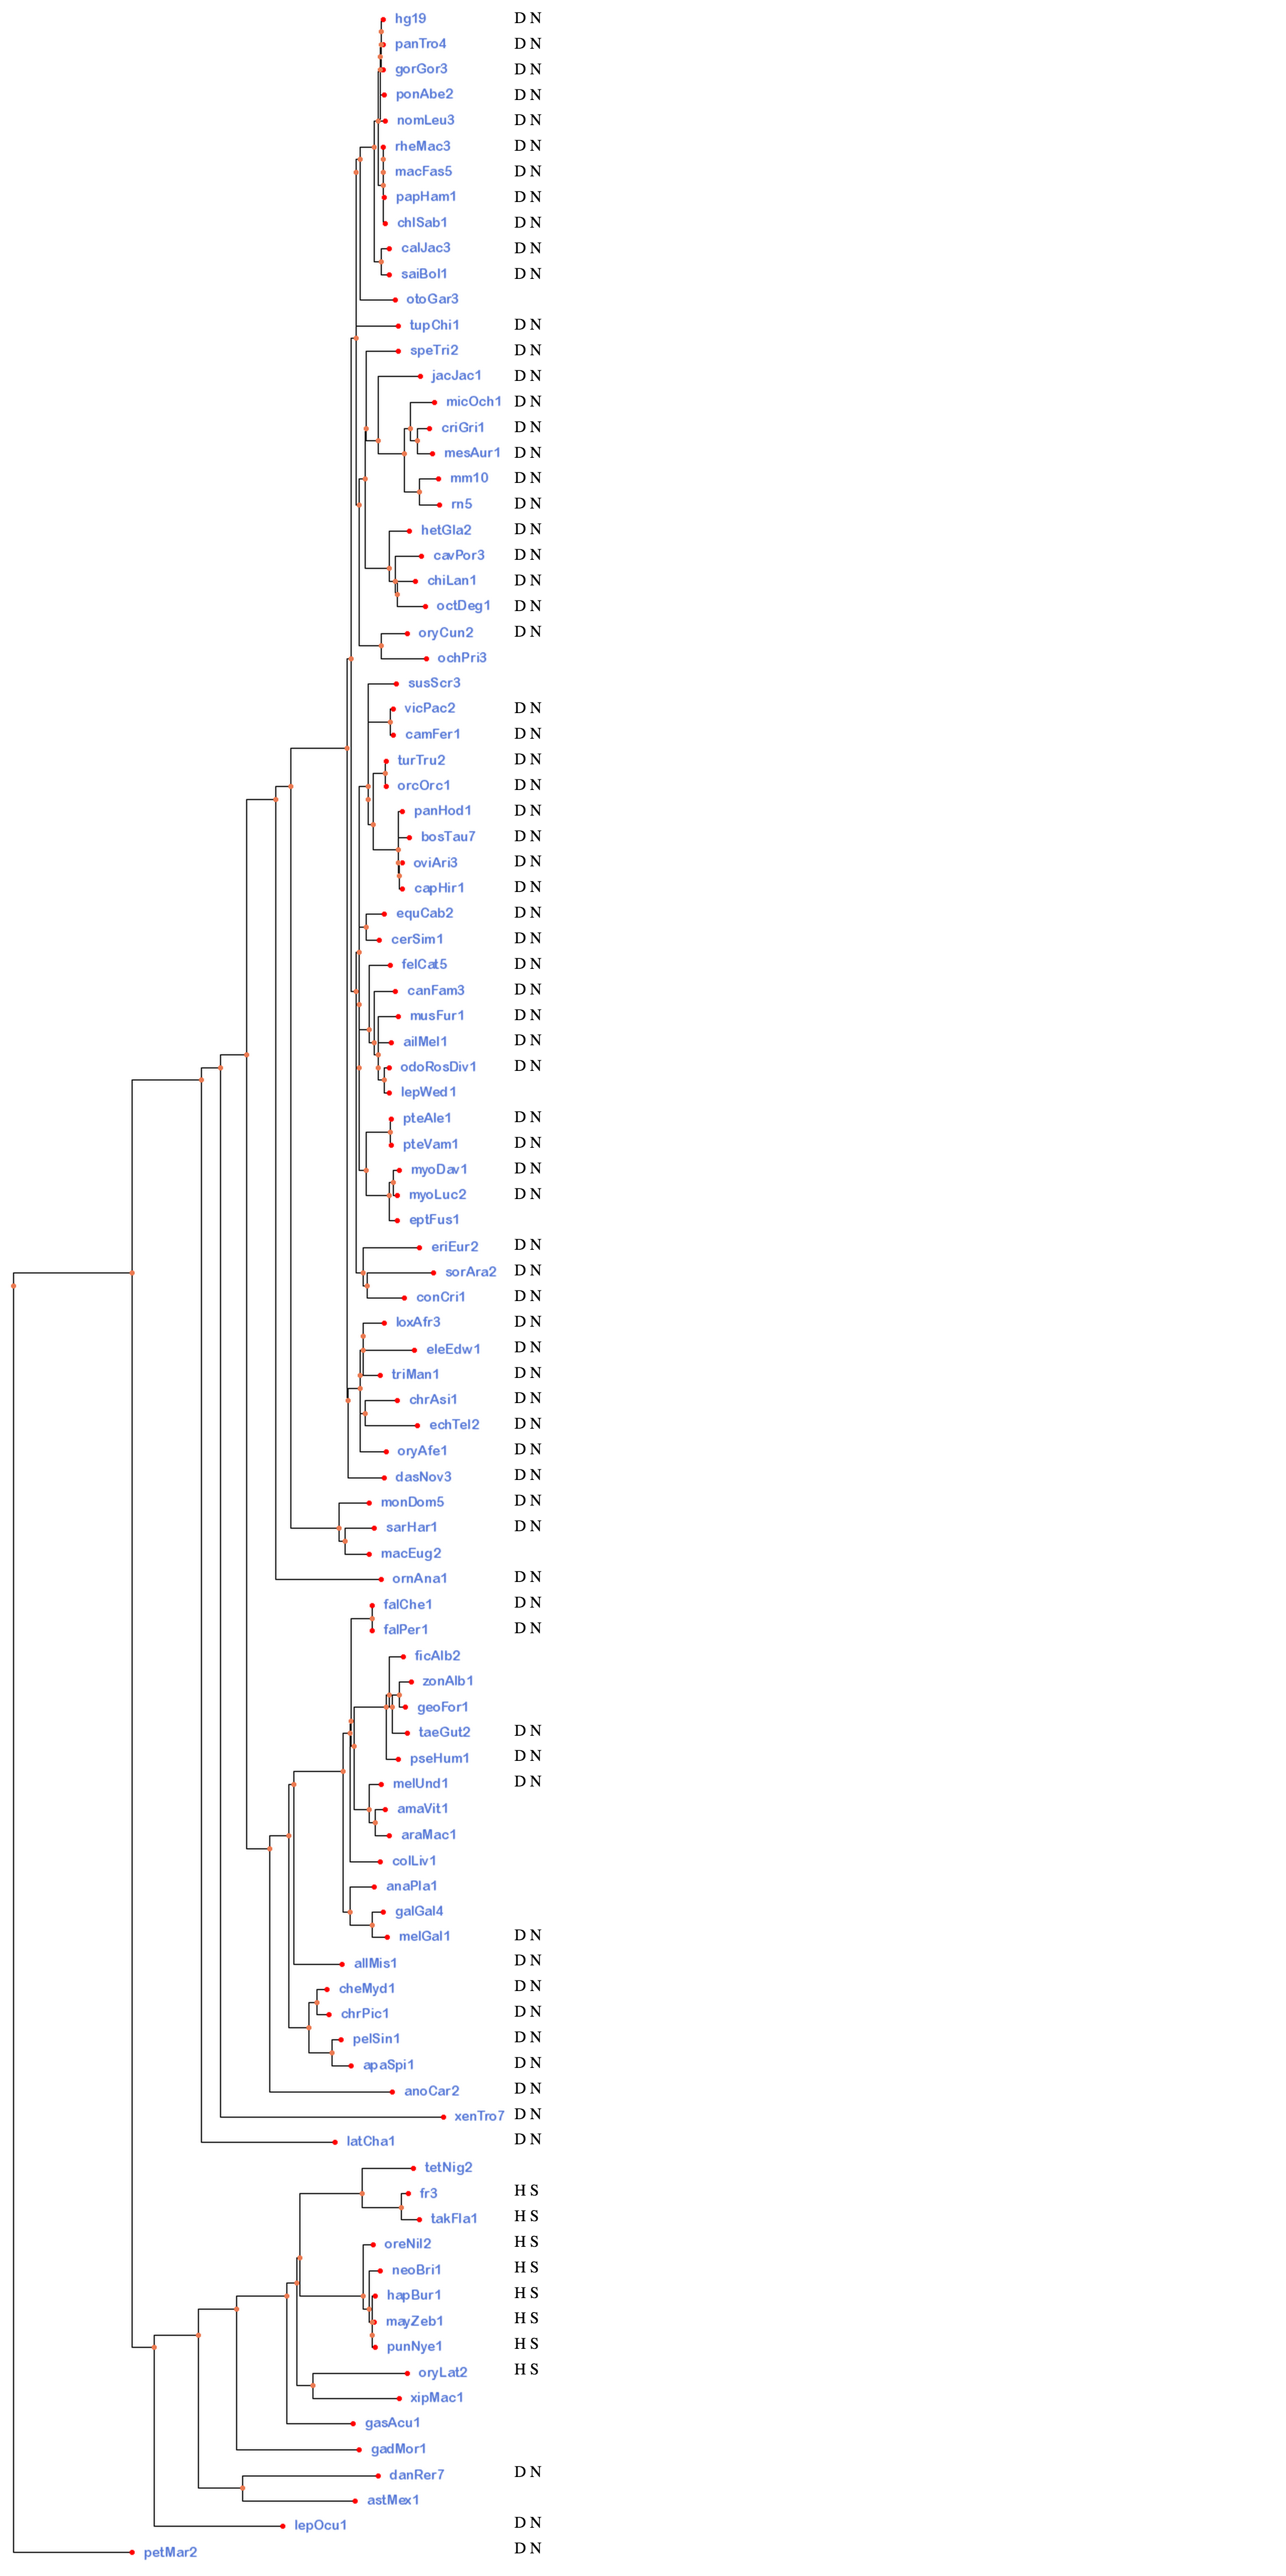
\includegraphics[height=17cm]{figs/gwas_figure_4_tree_coevolution.png}
  \label{fig:sub2}
\end{subfigure}
\FigureCaptionOpt{Example of amino acid interaction}{Example of interaction between amino acid \#441 of \textit{Senp1} and \#60 of \textit{Sumo1} proteins detected by our method with $\ell_C = 7.7$. Left: PDB structure 2G4D, shows that the amino acids are in close proximity. Right: Multiple sequence alignment and phylogenetic tree showing the putative compensatory amino acid substitution pair \texttt{D.N} replaced by \texttt{H.S}.}
\label{fig:gwas_jmol}
\end{figure}

Let the two proteins considered have amino acid sequences $A = a_1...a_m$ and $B = b_1...b_n$. 
To obtain the prediction score for this pair of proteins, we identify the pair of length-$k$ sub-strings $a_i, a_{i+1}, …, a_{i+k-1}$ and $b_j, b_{j+1}, …, b_{j+k-1}$ that exhibit the strongest support for parallel or anti-parallel interactions
\[
\ell_C(k) = \max\left[ \sum_{l=0}^{k-1}{ \ell_C[ MSA(a_{i+l}) , MSA(b_{j+l}) ]},  \sum_{l=0}^{k-1}{\ell_C[ MSA(a_{i+l}) , MSA(b_{j+k-1-l})} \right]
\]
\noindent where $k=3$ was determined empirically to provide the best predictive power. 
As shown in Figure \ref{fig:gwas_genegene}), prediction accuracy is quite good (p-value $< 2 \cdot 10^{-42}$), taking into account the modest amount of information considered by the model.

\subsection{Epistatic GWAS analysis}

We applied our methods to a cohort of $\sim 13,000$ individuals in a case-control study of type II diabetes \cite{mccarthy2015T2D}.
This multi-ethnic study covers exons of unrelated individuals from five major ancestral groups (European descent, South Asian, East Asian, Hispanic and African American descent) using an average sequencing coverage over $80 \times$, yielding $1.7$ million coding variants. 
The filters described in Methods section resulted in a number of variant pairs being analysed of less than $50$ million. 
By means of the z-score relationship between Bayes Factor and p-values shown in \cite{goodman1999toward}, we can set the GWAS significance threshold for $50$ million pairs at $log_{10}[BF_T] =  8.0$.

\paragraph{Results}
Variant annotated and filtered according to the previous paragraphs lead to variant pairs having high log likelihood in our logistic regression model  ($\ell_G > 6$, in equation \ref{eq:gwasLogLikLogReg}) that were further analysed under co-evolutionary and Bayesian models. 
The complete analysis took less than $2$ days using a $1,000$ CPU-cluster, thus showing that an epistatic GWAS analysis is feasible using current computational resources. 
Table \ref{tab:gwas_13k_results_1} shows the main results from our GWAS epistatic analysis, genes highlighted in red belong to a hand curated set of genes either associated with diabetes or known to be in diabetes related pathway. 
It should be noted that some of the top results include amino acid modification sites such as Phosphoserine (or Glycosylation, not shown), which are likely to be interaction loci.

\paragraph{Associations are purely epistatic}
In order to understand the nature of the putative epistatic associations, we compared our top epistatic GWAS results against a large single marker GWAS study of type II diabetes form the DIAGRAM consortia \cite{zeggini2008meta,voight2010twelve} as well as a meta analysis from the same consortia \cite{morris2012large}.
For each of our top $1,000$ results we looked up the closest entry from DIAGRAM dataset and analysed the corresponding p-values form all the three publicly released DIAGRAM datasets.

Only $14$ of the top $1,000$ results show suggestive association (p-value $\le 10^{-4}$) in a nearby loci (average distance $977$ bases).
Of these, only one of them is in our top 10 results (8:30982425\_T/G variant in \textit{WRN} gene has DIAGRAM p-value of $4.6 \times 10^{-4}$ and odds ratio $1.06$), whereas neither of the other suggestive single marker variants are our top 50 results.
This indicates that our top results are populated by pure epistatic putative effects having no marginal association with disease risk.
In light of this evidence, it should be noticed that \textit{conditional search} methods (based on selecting the top single marker results and performing epistatic analysis only this subset) would have missed most of our top results.
Likewise, an extension of that same limitation applies to our own method since we might be missing any three or higher order pure epistatic interaction, a limitation that doesn't seem to be plausible to overcome without introducing prior biological knowledge of interacting loci (which is obviously not available at the moment).

\figtab{gwas_13k_results_1}{gwas_13k_results_1}{14cm}{Results from epistatic GWAS analysis of type II diabetes sequencing data. First column shows total $log_{10}(BF_T)$; second and third columns show p-value and (raw) Bayes factor for logistic regression model. For each variant in the putative interaction pair: genomic coordinate, gene and functional annotation are shown. Genes marked in red are manually curated gene sets form diabetes related pathways}{Results from epistatic GWAS analysis of type II diabetes sequencing data}

\subsection{Power analysis}

In order to asses disease association power we performed extensive simulations.
As it is often the case in this kind of analysis some simplifying but realistic assumptions were required to make simulations computationally tractable. 
We assumed that: 
i) the disease has a logistic risk model;
ii) risk model has purely epistatic terms, this means that individual loci are assumed to have no marginal effect in disease risk;
iii) disease prevalence is $8\%$ according the well accepted prevalence for type II diabetes;
iv) cofactors influencing disease such as population admixture, age and sex were perfectly reduced by the model, meaning that no residual effects remains after correction;
v) genome wide significance was established as $0.05 / (10^6)^2 = 5 . 10^{-14}$;
and  
vi) that the study has an equal number of cases and controls.

Under these assumptions we calculated power by running $100$ iterations for every model having a combination of: 
i) sample sizes ranging from $10,000$ to $1,000,000$,
ii) log odds disease risk ranging from $0.1$ to $5$,
and 
iii) allele frequencies of each of the two loci ranging from $1\%$ to $20\%$.
Results for some selected models are shown in Figure \ref{fig:gwas_power}.

\fig{gwas_power}{gwas_power}{14cm}{Power calculation using a case/control pure two-loci epistatic model for disease prevalences of $8\%$ (type II diabetes). X-axis shows the number of samples in thousands (ranging from 10,000 to 1,000,000) and several joint risk values (from 0.1 to 5) are shown as different colors lines within each plot. Each plot represents a different allele frequencies combination (for each of the two loci), from top to bottom and left to right, the allele frequency value pairs are: $[AF_1=1\%, AF_2=1\%]$, $[AF_1=5\%, AF_2=1\%]$, $[AF_1=5\%, AF_2=2.5\%]$, $[AF_1=5\%, AF_2=5\%]$, $[AF_1=10\%, AF_2=1\%]$, $[AF_1=10\%, AF_2=2.5\%]$, $[AF_1=10\%, AF_2=5\%]$, $[AF_1=10\%, AF_2=7.5\%]$, $[AF_1=10\%, AF_2=10\%]$}{Power calculation using a pure two-loci epistatic model}

As expected these simulations show that very large sample sizes are required to find epistatic effects on rare variant loci (i.e. allele frequencies below $1\%$).
Even if risk is assumed to be over $2$, $3$, or $5$, sample sizes requirements are expected to be over $400,000$, $200,000$ and $100,000$ respectively (see Figure \ref{fig:gwas_power}, top-left plot).
For common variants (i.e. allele frequency of $5\%$) the sample sizes look more attainable in the near future, ranging from $10,000$ to $100,000$ samples when risk factors decrease from $5$ to $0.6$ (Figure \ref{fig:gwas_power}, middle row, left plot).
Finally, for relatively common variants (allele frequency of $10\%$) the sample sizes up to $100,000$ would be required for risk factors of $0.3$ which is still considered a high risk factor (Figure \ref{fig:gwas_power}, bottom right plot).

Unsurprisingly, our power calculation results show that large sample sizes are required in order to find epistatic interactions even under assumptions of relatively common variants and relatively high risk factors.
This highlights not only the complexity of finding epistatic genome wide associations but also how elusive these loci can be.

\paragraph{Power increase}
Finally it is worth mentioning that our epistatic GWAS method is able to increase power by using additional information from a co-evolutionary model.
According to our calculations, co-evolutionary information can increase Bayes Factor between $10^2$ and $10^4$, which is roughly equivalent to reducing genome wide association p-value threshold by two orders of magnitude \cite{goodman1999toward}, thus shifting the power curves in Figure \ref{fig:gwas_power} to the left.
Thus the net effect of adding information from a co-evolutionary model is to reduce sample size requirements roughly by half, which is quite remarkable given the little additional information being used by the model (only a multiple sequence alignment).

%---
\section{Discussion}
%---

In this paper, we propose a novel methodology for genome wide association studies of pairs of variants under putative epistatic interaction. 
Due to the large number of statistical tests required in an epistatic GWAS analysis and the corresponding reduction of statistical power, this type of analysis is meant to be applied to datasets consisting of large number of samples.
Our highly optimized algorithms are applicable to such large scale sequencing genomic studies and we show the application of our methods to a large scale exome sequencing study for type II diabetes consisting of $\sim 13,000$ samples and $\sim 1,7M$ variants. 
First, this shows that is is indeed feasible to apply our methods GWAS-scale datasets. 
Second, although larger cohorts are needed in order to find risk alleles that have lower frequencies and are not captured by this study, we show several suggestive association of pairs of putatively interacting variants with type II diabetes. 

The co-evolutionary model we propose in section \ref{sec:gwasQ2} requires multiple sequence alignment and the corresponding phylogenetic tree.
Intuitively, using an $MSA$ with larger number of sequences should improve co-evolutionary model detection and other co-evolutionary approaches indeed require very large $MSA$. 
Unfortunately, at this moment, $MSA$ consisting of a large number of sequences are available only for a small fraction of all human proteins and they often consist of a mixture of ortholog and paralog sequences which may lead to biases in co-evolutionary models. 
Furthermore, both the phylogenetic tree and the number of sequences in the $MSA$ should remain constant throughout the genome in order to take advantage of computational optimizations (matrix exponential pre-calculation and ``constant tree caching") that allow the algorithm to be applied at genome-wide scale. 
Many multiple sequence alignments (such as Pfam) have different number of sequences for each protein (thus different phylogenetic trees). This poses two main disadvantages for our methodology: 
i) we cannot benefit from the previously mentioned optimizations, since they require a constant phylogenetic tree throughout the whole genome; and 
ii) we would add the problem of reconciling different phylogenetic trees from two proteins, which may lead to inconsistencies. 
For all these reasons we selected UCSC's multi-100way \cite{karolchik2014ucsc}, a genome wide multiple sequence alignment of 100 organisms which has single genome wide phylogenetic tree. 
This $MSA$ is expected to grow with the advent of projects like G10K \cite{haussler2009genome} thus enabling more precise co-evolutionary predictions. 

In order to further validate our co-evolutionary model in the context of human disease, we tested whether it can separate clinically relevant variants from ClinVar database \cite{landrum2013clinvar} according to their clinical significance attribute (CLNSIG). 
Interestingly, variants categorized as ``benign" or ``druggable" have higher scores (mean $\ell_C$ within protein) than variants categorized as pathogenic (Supplementary Tables \ref{tab:gwas_clinvar}, \ref{tab:gwas_1Kg} and Figure \ref{fig:gwas_clinvar}). 
We speculate that this might be because amino acids that can be compensated would be characterized as ``benign" whereas deleterious amino acids changes cannot be compensated by mutations in other proteins. 

\paragraph{Comparison to other Co-Evolutionary methods}
There are several methodologies that can be used to predict putative interactions based on co-evolutionary theory.
Nevertheless most methods are limited respect to their applicability to GWAS-scale analyses:

\textit{Phylogenetic tree similarity} can be used as a proxy for the co-evolution of interacting proteins. 
Computational methods use matrix alignment \cite{ramani2003exploiting} which has demonstrated some degree of success. 
Unfortunately, such methods have two limiting factors: 
i) they require large (distinct) phylogenetic trees for each protein which are not be available for all proteins in the genome; and 
ii) use optimizations requiring long computational times to match matrices (e.g. simulated annealing) for each putative pair or proteins.

\textit{Correlation} methods aim to detect changes on one of the interacting proteins that are compensated by mutations in the other \cite{pazos1997correlated,gobel1994correlated}. 
Although these methods are fast enough to be applicable to GWAS scale studies, they still have at least two limitations: 
i) they require large number of sequences in the multiple sequence alignment to overcome noise (as we mentioned large MSAs are not be available throughout the whole genome); and 
ii) there are affected by biases mainly caused by phylogenetic tree and indirect correlations. 
  
\textit{Mutual information} methods share some similarities with correlation-based methods in the sense that are fast for GWAS studies but unfortunately they also require large MSAs and are well known for having bias caused by phylogenetic tree, and indirect correlations \cite{fares2006novel}.
There are methods based on mutual information than could perform some phylogenetic correction \cite{de2013emerging}, nevertheless they still require a large number of sequences in the MSA and are known to be biased by allele frequencies \cite{dunn2008mutual} which might limit their applicability for GWAS studies (particularly on non-common variants).
    
\textit{Global models} are designed to disentangle direct interactions from indirect ones. 
Several methods have been proposed which rely on: 
i) estimating parameters of Boltzmann distributions \cite{lapedes2012using,weigt2009identification}, 
ii) mean field approximations of Boltzmann distributions \cite{morcos2011direct}, 
iii) constrained optimizations for finding approximations of the inverses of large singular matrices \cite{jones2012psicov}, 
iv) marginalizing multidimensional extensions to mutual information \cite{clark2014multidimensional}; or 
v) solving a Bayesian network model \cite{burger2010disentangling}. 
All these models are so computationally heavy that can only be applied to very small sets of proteins. 
Furthermore, in some of the respective papers the authors mention that it is computationally infeasible to apply them to a single pair of proteins if the length is over a some low number of amino acids (e.g. $60$ \cite{weigt2009identification} or $500$ \cite{morcos2011direct}). 
It is therefore not possible to apply any of these method to GWAS-scale studies at the moment.

Our method attempts to solve two of the main problems common to some of the aforementioned methods: 
i) the requirement of large number of sequence, and 
ii) the phylogenetic bias.
These goals are achieved, at least partially, by using a well known Markov model of evolution.
It should be noted that until not long ago it was thought that methods based on Markov evolutionary theory were unsuitable for large scale studies \cite{de2013emerging}.

\paragraph{Comparison to other Epigenetic GWAS methods}
Although there large amounts of evidence supporting the theory that epistasis is ubiquitous, detecting epistatic interactions in human has been quite difficult and despite significant efforts the results have been scarce and difficult to reproduce \cite{zuk2012mystery}.

Many reasons have been given in this manuscript and elsewhere to indicate why detecting epistasis this is a very difficult task, with the most commonly cited one being the enormous number of statistical tests required, consequently having a significant reduction of statistical power and an increase in computational resources.
Thus methods based on exhaustive search can be computationally infeasible for all but very low order interactions analysis \cite{cordell2009detecting}.
Their counterpart are \textit{conditional search} methods \cite{li2011detecting} which are usually based on selecting the top single value associated variants and then performing epistatic analysis on a small subset.
Unfortunately these methods are guaranteed to ignore pure epistatic interactions and only detect marginal ones \cite{li2011detecting,cordell2002epistasis}.
Since there is no biological indication on whether complex traits have marginal or pure epistatic effects \cite{culverhouse2002perspective,zuk2012mystery,li2011detecting}, it might not be safe to rely on these type of methods when performing an unbiased association study.

Stochastic search based methods \cite{zhang2007bayesian} show great potential, but as far as we known they have not yet produced any significant results most likely due to small sample sizes used in the respective publications. 
Some authors pointed out that some of most well known methods in this family may have difficulties with large number of samples \cite{de2013emerging}.

Finally methods based machine learning have been proposed and applied with different degrees of success \cite{koo2013review, cordell2009detecting, li2011detecting}.
One of the main limitations of machine learning methods lies in the fact that the majority of them do not result in a statistical significance metric (such as p-value or Bayesian factor), thus researchers are often weary of conducting an expensive follow up studies based in results from machine learning algorithms.
Another limitation is that many machine learning approaches do not for allow appropriate correction from population admixture and other cofactors.

The methodology we proposed in this paper is based on a well established statistical procedures (Logistic Regression) using gold standard corrections for known population cofactors (eigen-analysis) as well as other disease cofactors (such age and sex are known to affect risk of type II diabetes).
Our method performs exhaustive search of second order interactions thus is capable of finding pure epistatic interactions pairs as well as marginal ones.
Finally, we address the power limitations by using co-evolutionary results from a well established Markov model of evolution and combining them with our association analysis by means of a Bayesian model.
This has the advantage that not only is being based on solid and well accepted theoretical grounds, but also it can increase statistical power and is capable of analysing large GWAS datasets that are becoming available now.

As a limitation, our methodology currently cannot analyse variants that are in complete LD.
There is evidence suggesting that genes relatively close (in genomic coordinates) tend to be correlated in expression (co-regulated) and likely to be in the same pathway or even to interact \cite{petkov2005evidence}.
Nevertheless it seems that complete LD would be a result of ``selective sweeps", in which an allele giving significant fitness advantage becomes more frequent so rapidly that there is little recombination.
These selective sweeps seem to be rare \cite{hernandez2011classic}, thus this limitation might not be encountered often in practice.

\paragraph{Future work}
We plan to extend our method to include context specific information by creating $Q_2$ estimates for different protein domains. 
This would allow to obtain better estimates for well characterized protein interaction regions. 
Another line of work is to perform GWAS using kernel based statistics of multiple variants \cite{wu2011rare} thus allowing simultaneous analysis of nearby variants in a putative interaction hotspot. 
In this case the epistatic information would be used as a function modifying the kernel, instead of a Bayesian prior.
It has also been suggested that positive selection might be used as an additional prior of epistatic interactions. 
Nevertheless a study comparing positive selection maps form 9 different methods \cite{akey2009constructing} shows that only $14\%$ of the regions have been identified in more than one study.
This striking lack of concordance suggests that using positive selection estimates would add more noise than information at this moment, although it is an interesting venue to explore when more reliable estimates become available.
